% Gabarit pandoc des corrigés publiés (brut et guidé). Contenu sans marque ni nom de site.
% Compilation : lualatex (latexmk -lualatex).
% Le Markdown reste la source unique : ne pas éditer ce fichier .tex à la main.
\documentclass[11pt,a4paper]{article}

% --- Moteur, polices (Latin Modern) et langue ---------------------------------
\usepackage{iftex}
\ifLuaTeX\else\errmessage{Ce document se compile avec lualatex}\fi
\usepackage{amsmath,amssymb,mathtools}
\usepackage{fontspec}
% mathrm=sym : \mathrm prend ses glyphes dans la police mathématique (ℓ, μ, Ω), comme KaTeX.
\usepackage[math-style=TeX,bold-style=TeX,mathrm=sym]{unicode-math}
% Repli pour les glyphes absents de Latin Modern (indices et exposants Unicode,
% flèches, filets des schémas en texte, symboles) : DejaVu, puis Latin Modern Math
% (ℓ, lettres mathématiques Unicode des légendes).
\directlua{
  luaotfload.add_fallback("repliTexte", {"DejaVuSerif:mode=harf;", "DejaVuSans:mode=harf;", "file:latinmodern-math.otf:mode=harf;"})
  luaotfload.add_fallback("repliMono", {"DejaVuSansMono:mode=harf;", "DejaVuSans:mode=harf;", "file:latinmodern-math.otf:mode=harf;"})
}
\setmainfont{Latin Modern Roman}[RawFeature={fallback=repliTexte}]
\setsansfont{Latin Modern Sans}[RawFeature={fallback=repliTexte}]
\setmonofont{Latin Modern Mono}[RawFeature={fallback=repliMono}]
\setmathfont{Latin Modern Math}
\usepackage[french]{babel}
\frenchsetup{SmallCapsFigTabCaptions=false}

% --- Mise en page --------------------------------------------------------------
\usepackage[a4paper,margin=2.2cm,headheight=14pt,footskip=1.2cm]{geometry}
\usepackage{microtype}
\setlength{\emergencystretch}{4em}
\tolerance=1500
\setlength{\parindent}{0pt}
\setlength{\parskip}{0.55\baselineskip plus 2pt minus 1pt}
\usepackage{xcolor}
% Gris nommés : babel-french rend « ! » actif dans le document.
\definecolor{gris2}{gray}{0.98}
\definecolor{gris3}{gray}{0.97}
\definecolor{gris5}{gray}{0.95}
\definecolor{gris35}{gray}{0.65}
\definecolor{gris40}{gray}{0.60}
\definecolor{gris45}{gray}{0.55}
\definecolor{gris50}{gray}{0.50}
\definecolor{gris55}{gray}{0.45}
\definecolor{gris60}{gray}{0.40}
\definecolor{gris65}{gray}{0.35}
\definecolor{gris70}{gray}{0.30}
\definecolor{gris80}{gray}{0.20}
\definecolor{gris85}{gray}{0.15}
\usepackage{graphicx}
\usepackage{float}
\usepackage{caption}
\captionsetup{font=small,labelformat=empty,justification=centering}
\usepackage{booktabs,longtable,array,multirow,calc}
\usepackage{siunitx}
\sisetup{locale=FR}
\usepackage[version=4]{mhchem}
\usepackage{listings}
\usepackage{fancyhdr}
\usepackage{lastpage}
\usepackage[most]{tcolorbox}
\usepackage{enumitem}
\setlist{nosep,leftmargin=*,topsep=2pt}
\usepackage[hidelinks,unicode]{hyperref}
\usepackage{bookmark}
\hypersetup{pdftitle={X-ENS PC — Mathématiques 2026},pdfauthor={Rédigé par IA},pdfcreator={LaTeX},pdfsubject={Corrigé brut}}
\usepackage{xurl}

% --- Pandoc : listes, tableaux, figures ----------------------------------------
\providecommand{\passthrough}[1]{#1}
\providecommand{\tightlist}{\setlength{\itemsep}{0pt}\setlength{\parskip}{0pt}}

\makeatletter
\def\maxwidth{\ifdim\Gin@nat@width>\linewidth\linewidth\else\Gin@nat@width\fi}
\def\maxheight{\ifdim\Gin@nat@height>0.55\textheight 0.55\textheight\else\Gin@nat@height\fi}
\makeatother
\setkeys{Gin}{width=\maxwidth,height=\maxheight,keepaspectratio}
\setcounter{secnumdepth}{-\maxdimen}
\providecommand{\pandocbounded}[1]{#1}

% --- Code (listings) -----------------------------------------------------------
\lstset{
  basicstyle=\ttfamily\small,
  columns=fullflexible,
  keepspaces=true,
  breaklines=true,
  breakatwhitespace=false,
  postbreak=\mbox{\textcolor{gris50}{$\hookrightarrow$}\space},
  frame=single,
  rulecolor=\color{gris35},
  framesep=4pt,
  xleftmargin=5pt,xrightmargin=5pt,
  backgroundcolor=\color{gris3},
  keywordstyle=\bfseries,
  commentstyle=\color{gris65},
  stringstyle=\color{gris80},
  showstringspaces=false,
  tabsize=4,
  extendedchars=true,
  aboveskip=6pt,belowskip=6pt,
}

% --- Macros des corrigés (KaTeX ↔ LaTeX) ---------------------------------------
% Les corrigés sont écrits pour KaTeX : on définit ici ce que KaTeX connaît et
% que LaTeX n'a pas, sans jamais retoucher le Markdown.
\providecommand{\R}{\mathbb{R}}
\providecommand{\N}{\mathbb{N}}
\providecommand{\Z}{\mathbb{Z}}
\providecommand{\Q}{\mathbb{Q}}
\providecommand{\C}{\mathbb{C}}
\providecommand{\dd}{\mathrm{d}}
\providecommand{\llbracket}{\lBrack}
\providecommand{\rrbracket}{\rBrack}
\providecommand{\lBrace}{\lbrace}
\providecommand{\rBrace}{\rbrace}
\providecommand{\Box}{\square}
\providecommand{\Diamond}{\lozenge}
\providecommand{\varnothing}{\emptyset}
\providecommand{\argmax}{\operatorname*{arg\,max}}
\providecommand{\argmin}{\operatorname*{arg\,min}}
\renewcommand{\leq}{\leqslant}
\renewcommand{\geq}{\geqslant}

% Équation hors texte : réduite à la largeur de la ligne si elle déborde.
\newsavebox{\boiteequation}
\newcommand{\equationajustee}[1]{%
  \sbox{\boiteequation}{$\displaystyle #1$}%
  \ifdim\wd\boiteequation>\linewidth
    \[\resizebox{\linewidth}{!}{\usebox{\boiteequation}}\]%
  \else
    \[#1\]%
  \fi}

% --- Encadrés pédagogiques (sobres, lisibles en noir et blanc) -----------------
\tcbset{
  encadre/.style={
    enhanced,breakable,sharp corners,
    colback=white,colframe=gris55,
    boxrule=0.4pt,leftrule=2.2pt,
    left=6pt,right=6pt,top=3pt,bottom=3pt,
    before skip=6pt,after skip=6pt,
    fonttitle=\bfseries\small,coltitle=black,
    attach title to upper,after title={\quad},
    parbox=false,
  }
}
\newtcolorbox{indication}[1]{encadre,colframe=gris45,colback=gris2,title={Indication~#1}}
\newtcolorbox{methode}{encadre,colframe=gris70,title={Méthode}}
\newtcolorbox{piege}{encadre,colframe=gris85,boxrule=0.8pt,leftrule=2.2pt,title={Piège}}
\newtcolorbox{jury}{encadre,colframe=gris60,colback=gris5,title={Jury}}
\newtcolorbox{encadrenote}{encadre,colframe=gris40}

% --- Titres de section ---------------------------------------------------------
\usepackage{titlesec}
\titleformat{\section}{\Large\bfseries}{}{0pt}{}
\titleformat{\subsection}{\large\bfseries}{}{0pt}{}
\titleformat{\subsubsection}{\normalsize\bfseries}{}{0pt}{}
\titlespacing*{\section}{0pt}{14pt plus 4pt minus 2pt}{6pt}
\titlespacing*{\subsection}{0pt}{10pt plus 3pt minus 2pt}{4pt}
\titlespacing*{\subsubsection}{0pt}{8pt plus 2pt minus 2pt}{2pt}

% --- En-tête et pied de page ---------------------------------------------------
\pagestyle{fancy}
\fancyhf{}
\fancyhead[L]{\small\textsc{Corrigé brut} · X-ENS PC}
\fancyhead[R]{\small Maths PC 2026}
\fancyfoot[L]{\footnotesize Corrigé rédigé par IA, non officiel}
\fancyfoot[R]{\footnotesize \thepage\,/\,\pageref*{LastPage}}
\renewcommand{\headrulewidth}{0.4pt}
\renewcommand{\footrulewidth}{0pt}
\fancypagestyle{plain}{\fancyhf{}\fancyfoot[R]{\footnotesize \thepage\,/\,\pageref*{LastPage}}\fancyfoot[L]{\footnotesize Corrigé rédigé par IA, non officiel}\renewcommand{\headrulewidth}{0pt}}

\begin{document}
\thispagestyle{plain}
\begin{center}
  {\small\scshape Corrigé brut}\par\smallskip
  {\LARGE\bfseries X-ENS PC — Mathématiques 2026\par}\medskip
  {\large X-ENS · PC · Maths PC · 2026\par}
\end{center}
\vspace{2pt}\hrule\vspace{8pt}

\emph{Corrigé rédigé par IA, non officiel. Signalez toute erreur.}

Épreuve n° 1 de la filière PC, durée 4 h, calculatrice interdite. Notations du sujet : \(\operatorname{ch},\operatorname{sh},\operatorname{th}\), le produit scalaire usuel \(x\cdot y\) de \(\mathbb R^d\), et \(\phi(\lambda)=\ln E[e^{\lambda\cdot X}]\).

\textbf{Erratum de l'énoncé (question 21).} Avec la fonction \(I\) de l'énoncé, la limite de la question 21 vaut \(I(x)+\ln 2\), et non \(I(x)\) : il manque un terme constant en \(\ln 2\), ce que confirme le rapport du jury. De même, la convergence admise après la question 22 s'écrit en toute rigueur
\equationajustee{G_N(\beta,h)\xrightarrow[N\to+\infty]{}g(\beta,h)-\ln 2 .}
On démontre la forme exacte en Q21 et on en tient compte en Q30. Les questions 23 à 29, 31 et 32 ne portent que sur \(\psi''_{\beta,h}\), sur les points de maximum de \(\psi_{\beta,h}\) ou sur des différences de valeurs de \(g\) : elles ne dépendent pas de cette constante.

\textbf{Coquille (question 5).} Il faut lire « en tout point \(x\in\mathbb R^d\) ».

\begin{center}\rule{0.5\linewidth}{0.5pt}\end{center}

\hypertarget{premiuxe8re-partie}{%
\section{Première partie}\label{premiuxe8re-partie}}

\hypertarget{question-1}{%
\subsection{Question 1}\label{question-1}}

Soit \(h>0\). Pour \(0<s\leqslant t\), posons \(\alpha=s/t\in\,]0,1]\). On a \(x+s=\alpha(x+t)+(1-\alpha)x\), donc, par la définition de la convexité,
\equationajustee{g(x+s)\leqslant\alpha\,g(x+t)+(1-\alpha)\,g(x).}
En retranchant \(g(x)\) et en divisant par \(s>0\) :
\equationajustee{\frac{g(x+s)-g(x)}{s}\leqslant\frac{g(x+t)-g(x)}{t}.}
Le taux \(\tau_+(s)=\frac{g(x+s)-g(x)}{s}\) est donc croissant sur \(]0,+\infty[\).

De même, \(x-s=\alpha(x-t)+(1-\alpha)x\) donne
\equationajustee{g(x-s)-g(x)\leqslant\frac st\big(g(x-t)-g(x)\big).}
Après division par \(s\) et changement de signe, le taux \(\tau_-(s)=\frac{g(x)-g(x-s)}{s}\) est \textbf{décroissant} en \(s\).

Comme \(g\) est dérivable en \(x\) (et seulement supposée telle en ce point), \(\tau_+(s)\) et \(\tau_-(s)\) tendent vers \(g'(x)\) quand \(s\to0^+\).

Pour \(0<s\leqslant h\), la monotonie donne
\equationajustee{\tau_-(h)\leqslant\tau_-(s)\qquad\text{et}\qquad\tau_+(s)\leqslant\tau_+(h).}
Dans chacune de ces inégalités, le membre de gauche et le membre de droite ont une limite quand \(s\to0^+\) (l'un est constant). Le passage à la limite dans les inégalités larges donne \(\tau_-(h)\leqslant g'(x)\) et \(g'(x)\leqslant\tau_+(h)\) :
\equationajustee{\boxed{\frac{g(x)-g(x-h)}{h}\leqslant g'(x)\leqslant\frac{g(x+h)-g(x)}{h}}}

\begin{figure}[H]
\centering
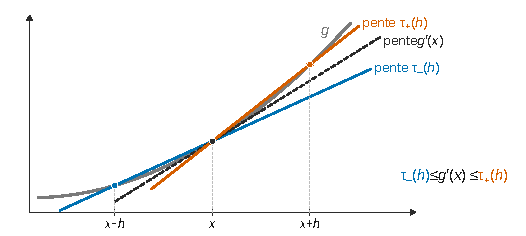
\includegraphics{figures/q01-pentes-cordes.pdf}
\caption*{Figure 1 --- Inégalité des pentes : pour g convexe, la corde de gauche
(pente τ₋(h)) est moins inclinée que la tangente en x, elle-même moins
inclinée que la corde de droite (pente τ₊(h))}
\end{figure}

\hypertarget{question-2}{%
\subsection{Question 2}\label{question-2}}

Soient \(x,y\in\mathbb R\) et \(\alpha\in[0,1]\). Pour tout \(n\),
\equationajustee{f_n(\alpha x+(1-\alpha)y)\leqslant\alpha f_n(x)+(1-\alpha)f_n(y).}
Les trois suites \((f_n(\alpha x+(1-\alpha)y))_n\), \((f_n(x))_n\) et \((f_n(y))_n\) convergent, par convergence simple. Le passage à la limite dans l'inégalité large donne
\equationajustee{f(\alpha x+(1-\alpha)y)\leqslant\alpha f(x)+(1-\alpha)f(y).}
\textbf{\(f\) est convexe.}

\hypertarget{question-3}{%
\subsection{Question 3}\label{question-3}}

Pour \(n\in\mathbb N\), posons \(f_n(x)=\sqrt{x^2+\frac1{n+1}}\). Le radicande est minoré par \(\frac1{n+1}>0\).

La racine carrée est de classe \(\mathcal C^\infty\) sur \(]0,+\infty[\), donc \(f_n\) est de classe \(\mathcal C^2\) sur \(\mathbb R\), avec
\equationajustee{f_n'(x)=\frac{x}{\sqrt{x^2+\frac1{n+1}}}}
et
\equationajustee{f_n''(x)=\frac{\frac1{n+1}}{\big(x^2+\frac1{n+1}\big)^{3/2}}>0 .}

\emph{Convexité.} La hessienne de \(f_n\) (matrice \(1\times1\) égale à \(f_n''(x)\)) est symétrique positive en tout point. Par Q6 avec \(d=1\), \textbf{\(f_n\) est convexe} ; elle est dérivable.

\emph{Convergence.} Pour \(x\) fixé, \(x^2+\frac1{n+1}\to x^2\) et la racine carrée est continue sur \([0,+\infty[\), donc \(f_n(x)\to\sqrt{x^2}=|x|\).

\textbf{La limite simple \(f=|\cdot|\) n'est pas dérivable en \(0\)} : son taux d'accroissement en \(0\) vaut \(1\) à droite et \(-1\) à gauche.

\hypertarget{question-4}{%
\subsection{Question 4}\label{question-4}}

Soit \(\varepsilon>0\). Comme \(f\) est dérivable en \(x\), on fixe \(h>0\) tel que
\equationajustee{\frac{f(x)-f(x-h)}{h}\geqslant f'(x)-\varepsilon}
et
\equationajustee{\frac{f(x+h)-f(x)}{h}\leqslant f'(x)+\varepsilon.}
Le pas \(h\) étant fixé, la convergence simple en \(x-h\), \(x\) et \(x+h\) fournit \(n_0\) tel que, pour \(n\geqslant n_0\),
\equationajustee{\frac{f_n(x)-f_n(x-h)}{h}\geqslant\frac{f(x)-f(x-h)}{h}-\varepsilon}
et
\equationajustee{\frac{f_n(x+h)-f_n(x)}{h}\leqslant\frac{f(x+h)-f(x)}{h}+\varepsilon.}
La question 1, appliquée à \(f_n\) (convexe et dérivable en \(x\)), encadre \(f_n'(x)\) entre ces deux taux. On enchaîne les minorations d'une part, les majorations d'autre part : pour \(n\geqslant n_0\),
\equationajustee{\begin{aligned}
f_n'(x)&\geqslant\frac{f_n(x)-f_n(x-h)}{h}\geqslant f'(x)-2\varepsilon,\\
f_n'(x)&\leqslant\frac{f_n(x+h)-f_n(x)}{h}\leqslant f'(x)+2\varepsilon.
\end{aligned}}
Ainsi \(|f_n'(x)-f'(x)|\leqslant2\varepsilon\) pour \(n\geqslant n_0\). Ceci établit à la fois l'existence de la limite et sa valeur :
\equationajustee{\boxed{\lim_{n\to\infty}f_n'(x)=f'(x)}}

\hypertarget{question-5}{%
\subsection{Question 5}\label{question-5}}

(On lit \(x\in\mathbb R^d\).) Rappelons qu'une matrice \(S\in\mathcal M_d(\mathbb R)\) est symétrique positive si \({}^tS=S\) et \({}^tu\,S\,u\geqslant0\) pour tout \(u\in\mathbb R^d\).

\emph{Symétrie.} \(g\) étant de classe \(\mathcal C^2\), sa hessienne \(\nabla^2g(x)\) est symétrique (théorème de Schwarz).

\emph{Positivité.} Soit \(u\in\mathbb R^d\) et \(\gamma(t)=g(x+tu)\), de classe \(\mathcal C^2\) sur \(\mathbb R\). Par la règle de la chaîne,
\equationajustee{\gamma'(t)=\sum_{i=1}^du_i\,\partial_ig(x+tu)}
et
\equationajustee{\begin{aligned}
\gamma''(t)&=\sum_{i,j}u_iu_j\,\partial_{ij}g(x+tu)\\
&={}^tu\,\nabla^2g(x+tu)\,u.
\end{aligned}}
\(\gamma\) est convexe, car \(x+(\alpha s+(1-\alpha)t)u=\alpha(x+su)+(1-\alpha)(x+tu)\).

Pour \(s<t\), la question 1 appliquée à \(\gamma\) en \(s\) et en \(t\), avec le pas \(t-s\), donne
\equationajustee{\gamma'(s)\leqslant\frac{\gamma(t)-\gamma(s)}{t-s}\leqslant\gamma'(t).}
\(\gamma'\) est donc croissante, d'où \(\gamma''\geqslant0\). En \(t=0\), \({}^tu\,\nabla^2g(x)\,u\geqslant0\) pour tout \(u\).

\textbf{La hessienne de \(g\) en \(x\) est symétrique positive.}

\hypertarget{question-6}{%
\subsection{Question 6}\label{question-6}}

Soient \(x,y\in\mathbb R^d\) et \(\gamma(t)=g(x+t(y-x))\) pour \(t\in[0,1]\). Il suffit d'établir \(\gamma(\alpha)\leqslant\alpha\gamma(1)+(1-\alpha)\gamma(0)\) pour tout \(\alpha\in[0,1]\). Comme en Q5,
\equationajustee{\gamma''(t)={}^t(y-x)\,\nabla^2g\big(x+t(y-x)\big)\,(y-x)\geqslant0,}
donc \(\gamma'\) est croissante sur \([0,1]\).

Soit donc \(\alpha\in[0,1]\). Si \(\alpha\in\{0,1\}\), l'inégalité cherchée est une égalité. Sinon, le théorème des accroissements finis sur \([0,\alpha]\) et sur \([\alpha,1]\) fournit \(c_1\in\,]0,\alpha[\) et \(c_2\in\,]\alpha,1[\) tels que
\equationajustee{\begin{aligned}
\frac{\gamma(\alpha)-\gamma(0)}{\alpha}&=\gamma'(c_1)\\
&\leqslant\gamma'(c_2)\\
&=\frac{\gamma(1)-\gamma(\alpha)}{1-\alpha}.
\end{aligned}}
En multipliant par \(\alpha(1-\alpha)>0\) :
\equationajustee{\begin{aligned}
(1-\alpha)\big(\gamma(\alpha)-\gamma(0)\big)&\leqslant\alpha\big(\gamma(1)-\gamma(\alpha)\big),\\
\gamma(\alpha)&\leqslant\alpha\,\gamma(1)+(1-\alpha)\,\gamma(0).
\end{aligned}}
Ainsi \(g(\alpha y+(1-\alpha)x)\leqslant\alpha g(y)+(1-\alpha)g(x)\) : \textbf{\(g\) est convexe.}

\hypertarget{question-7}{%
\subsection{Question 7}\label{question-7}}

Soit \(V\subset\mathbb R^d\) l'ensemble \textbf{fini} des valeurs de \(X\) et \(p_v=P[X=v]\). Par la formule de transfert,
\equationajustee{Z(\lambda)=E[e^{\lambda\cdot X}]=\sum_{v\in V}p_v\,e^{\lambda\cdot v}.}
C'est une somme finie de fonctions \(\mathcal C^\infty\) de \(\lambda\).

De plus \(Z>0\) : les poids \(p_v\) sont positifs de somme \(1\) et les exponentielles sont strictement positives. Donc \(\phi=\ln\circ Z\) est de classe \(\mathcal C^\infty\), en particulier \(\mathcal C^2\).

Une somme finie se dérive terme à terme :
\equationajustee{\begin{aligned}
\partial_iZ(\lambda)&=\sum_vp_v\,v_i\,e^{\lambda\cdot v}=E[X_ie^{\lambda\cdot X}],\\
\partial_{ij}Z(\lambda)&=\sum_vp_v\,v_iv_j\,e^{\lambda\cdot v}=E[X_iX_je^{\lambda\cdot X}].
\end{aligned}}
On en déduit
\equationajustee{\begin{aligned}
\partial_i\phi&=\frac{\partial_iZ}{Z},\\
\partial_{ij}\phi&=\frac{\partial_{ij}Z}{Z}-\frac{\partial_iZ\,\partial_jZ}{Z^2},
\end{aligned}}
c'est-à-dire
\equationajustee{\boxed{\begin{aligned}
\frac{\partial\phi}{\partial\lambda_i}(\lambda)&=\frac{E[X_ie^{\lambda\cdot X}]}{E[e^{\lambda\cdot X}]},\\
\frac{\partial^2\phi}{\partial\lambda_i\partial\lambda_j}(\lambda)&=\frac{E[X_iX_je^{\lambda\cdot X}]}{E[e^{\lambda\cdot X}]}-\frac{E[X_ie^{\lambda\cdot X}]}{E[e^{\lambda\cdot X}]}\,\frac{E[X_je^{\lambda\cdot X}]}{E[e^{\lambda\cdot X}]}
\end{aligned}}}

\hypertarget{question-8}{%
\subsection{Question 8}\label{question-8}}

Fixons \(\lambda\) et posons \(q_v=p_v\,e^{\lambda\cdot v}/Z(\lambda)\) : \(q_v\geqslant0\) et \(\sum_vq_v=1\). Notons \(\langle f\rangle=\sum_vq_vf(v)\) pour \(f:V\to\mathbb R\). D'après Q7,
\equationajustee{\partial_{ij}\phi(\lambda)=\langle v_iv_j\rangle-\langle v_i\rangle\langle v_j\rangle .}
Cette expression est symétrique en \((i,j)\) : la hessienne \(\nabla^2\phi(\lambda)\) est symétrique. Pour \(u\in\mathbb R^d\), par bilinéarité,
\equationajustee{\begin{aligned}
{}^tu\,\nabla^2\phi(\lambda)\,u&=\big\langle(u\cdot v)^2\big\rangle-\langle u\cdot v\rangle^2\\
&=\big\langle(u\cdot v-\langle u\cdot v\rangle)^2\big\rangle\\
&\geqslant0 .
\end{aligned}}
La hessienne de \(\phi\) est donc symétrique positive en tout point, et \(\phi\) est de classe \(\mathcal C^2\) (Q7). Par Q6, \textbf{\(\phi\) est convexe.}

\begin{center}\rule{0.5\linewidth}{0.5pt}\end{center}

\hypertarget{deuxiuxe8me-partie}{%
\section{Deuxième partie}\label{deuxiuxe8me-partie}}

\hypertarget{question-9}{%
\subsection{Question 9}\label{question-9}}

\(H_N(0,h,a)=h\sum_ia_i\). Les variables \(e^{h\sigma_1},\dots,e^{h\sigma_N}\) sont mutuellement indépendantes (fonctions de variables indépendantes), donc
\equationajustee{\begin{aligned}
Z_N(0,h)&=E\Big[\prod_{i=1}^Ne^{h\sigma_i}\Big]\\
&=\prod_{i=1}^NE[e^{h\sigma_i}]\\
&=\Big(\frac{e^h+e^{-h}}2\Big)^N\\
&=\operatorname{ch}(h)^N .
\end{aligned}}
D'où \(\boxed{Z_{N+1}(0,h)=\operatorname{ch}(h)Z_N(0,h)}\) et \(\boxed{F_N(0,h)=\ln\operatorname{ch}(h)}\).

\hypertarget{question-10}{%
\subsection{Question 10}\label{question-10}}

Posons
\equationajustee{\begin{aligned}
Y^{(N)}&=\big(Y^{(N)}_1,Y^{(N)}_2\big),\\
Y^{(N)}_1&=\sum_{i=1}^{N-1}\sigma_i\sigma_{i+1}+\sigma_N\sigma_1,\\
Y^{(N)}_2&=\sum_{i=1}^N\sigma_i .
\end{aligned}}
C'est une variable aléatoire à valeurs dans un sous-ensemble \textbf{fini} de \(\mathbb R^2\) (au plus \(2^N\) valeurs). Pour \(\lambda=(\beta,h)\), on a \(H_N(\beta,h,X^{(N)})=\lambda\cdot Y^{(N)}\), donc
\equationajustee{\ln Z_N(\beta,h)=\ln E\big[e^{\lambda\cdot Y^{(N)}}\big]=\phi_{Y^{(N)}}(\lambda).}
Par Q8 appliquée à \(X=Y^{(N)}\) et \(d=2\), cette fonction est convexe sur \(\mathbb R^2\). Multiplier par \(\frac1N>0\) conserve la convexité : \textbf{\(F_N\) est convexe sur \(\mathbb R^2\).}

\hypertarget{question-11}{%
\subsection{Question 11}\label{question-11}}

On calcule
\equationajustee{\begin{aligned}
\operatorname{tr}A&=e^{\beta-h}+e^{\beta+h}=2e^\beta\operatorname{ch}h,\\
\det A&=e^{2\beta}-e^{-2\beta}=2\operatorname{sh}(2\beta).
\end{aligned}}
Le polynôme caractéristique \(\chi_A(t)=t^2-2e^\beta\operatorname{ch}(h)\,t+2\operatorname{sh}(2\beta)\) a pour discriminant
\equationajustee{\begin{aligned}
\Delta&=4\big(e^{2\beta}\operatorname{ch}^2h-e^{2\beta}+e^{-2\beta}\big)\\
&=4\big(e^{2\beta}\operatorname{sh}^2h+e^{-2\beta}\big),
\end{aligned}}
grâce à \(\operatorname{ch}^2h-1=\operatorname{sh}^2h\). Comme \(e^{-2\beta}>0\), on a \(\Delta>0\) : \(\chi_A\) a deux racines réelles distinctes, qui sont les deux valeurs propres de \(A\). La plus grande est
\equationajustee{\boxed{\begin{aligned}
\lambda(\beta,h)&=e^\beta\operatorname{ch}(h)+\sqrt{e^{2\beta}\operatorname{ch}^2(h)-2\operatorname{sh}(2\beta)}\\
&=e^\beta\operatorname{ch}(h)+\sqrt{e^{2\beta}\operatorname{sh}^2(h)+e^{-2\beta}}
\end{aligned}}}

\hypertarget{question-12}{%
\subsection{Question 12}\label{question-12}}

Par définition, \(B_{a_i,a_{i+1}}=\exp(\beta a_ia_{i+1}+ha_i)\) et \(B_{a_N,a_1}=\exp(\beta a_Na_1+ha_N)\). Un produit d'exponentielles est l'exponentielle de la somme :
\equationajustee{\begin{aligned}
\Big(\prod_{i=1}^{N-1}B_{a_i,a_{i+1}}\Big)B_{a_N,a_1}&=\exp\Big(\sum_{i=1}^{N-1}(\beta a_ia_{i+1}+ha_i)+\beta a_Na_1+ha_N\Big)\\
&=\exp\Big(\beta\sum_{i=1}^{N-1}a_ia_{i+1}+\beta a_Na_1+h\sum_{i=1}^Na_i\Big),
\end{aligned}}
qui est \(\exp(H_N(\beta,h,a))\).

\begin{figure}[H]
\centering
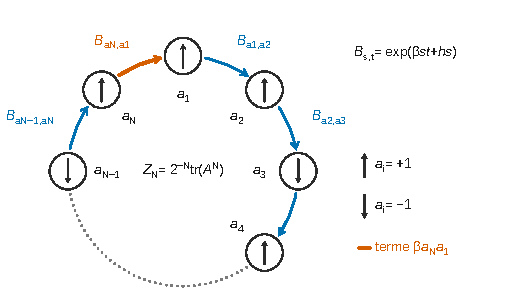
\includegraphics{figures/q12-anneau-transfert.pdf}
\caption*{Figure 2 --- Anneau de spins : chaque lien orienté aᵢ → aᵢ₊₁ porte le
facteur B(aᵢ, aᵢ₊₁), et le terme β a\_N a₁ referme la chaîne, d'où une
trace}
\end{figure}

\hypertarget{question-13}{%
\subsection{Question 13}\label{question-13}}

\(X^{(N)}\) est uniforme sur \(\{-1,1\}^N\) : par indépendance, chaque configuration \(a\) a la probabilité \(2^{-N}\). Par la formule de transfert et Q12,
\equationajustee{Z_N(\beta,h)=2^{-N}\sum_{a\in\{-1,1\}^N}\Big(\prod_{i=1}^{N-1}B_{a_i,a_{i+1}}\Big)B_{a_N,a_1}.}
(Les facteurs \(B_{\sigma_i,\sigma_{i+1}}\) ne sont pas indépendants : on ne factorise pas l'espérance, on la développe en somme sur les configurations.)

Indexons lignes et colonnes par \((-1,+1)\), dans cet ordre. La matrice \(B=(B_{s,t})\) vaut
\equationajustee{B=\begin{pmatrix}e^{\beta-h}&e^{-\beta-h}\\e^{-\beta+h}&e^{\beta+h}\end{pmatrix}={}^tA .}
Par la formule du produit matriciel,
\equationajustee{(B^N)_{a_1,a_1}=\sum_{a_2,\dots,a_N}B_{a_1,a_2}B_{a_2,a_3}\cdots B_{a_{N-1},a_N}B_{a_N,a_1}.}
En sommant sur \(a_1\), la somme sur les configurations vaut \(\operatorname{tr}(B^N)\). Enfin \(\operatorname{tr}(B^N)=\operatorname{tr}\big({}^t(A^N)\big)=\operatorname{tr}(A^N)\). Donc
\equationajustee{\boxed{Z_N(\beta,h)=2^{-N}\operatorname{tr}(A^N)}}

\hypertarget{question-14}{%
\subsection{Question 14}\label{question-14}}

Soit \(\mu\) l'autre valeur propre de \(A\) et \(\lambda=\lambda(\beta,h)\). \(A\) est diagonalisable (deux valeurs propres distinctes en dimension 2), donc \(\operatorname{tr}(A^N)=\lambda^N+\mu^N\).

\emph{Comparaison des modules.} \(\lambda>0\), comme somme de \(e^\beta\operatorname{ch}h>0\) et d'une racine carrée.

Pour \(\beta\geqslant0\), \(\lambda\mu=\det A=2\operatorname{sh}(2\beta)\geqslant0\), donc \(\mu\geqslant0\).

Comme \(\mu<\lambda\) (valeurs propres distinctes, \(\lambda\) la plus grande), on obtient \(0\leqslant\mu/\lambda<1\).

Alors
\equationajustee{F_N(\beta,h)=\ln\lambda-\ln2+\frac1N\ln\Big(1+\big(\tfrac\mu\lambda\big)^N\Big),}
avec
\equationajustee{0\leqslant\frac1N\ln\Big(1+\big(\tfrac\mu\lambda\big)^N\Big)\leqslant\frac{\ln2}N .}
Par encadrement,
\equationajustee{\boxed{\lim_{N\to+\infty}F_N(\beta,h)=\ln\lambda(\beta,h)-\ln2}}

\hypertarget{question-15}{%
\subsection{Question 15}\label{question-15}}

D'après Q11, \(\lambda(\beta,h)=e^\beta\operatorname{ch}h+\sqrt{R(\beta,h)}\) avec
\equationajustee{R(\beta,h)=e^{2\beta}\operatorname{sh}^2h+e^{-2\beta}.}
\(R\) est de classe \(\mathcal C^\infty\) sur \(\mathbb R^2\) (sommes, produits et composées de fonctions \(\mathcal C^\infty\)), et \(R\geqslant e^{-2\beta}>0\).

La racine carrée est \(\mathcal C^\infty\) sur \(]0,+\infty[\), donc \(\sqrt R\) l'est aussi.

\textbf{\(\lambda\) est de classe \(\mathcal C^\infty\) sur \(\mathbb R^2\)}, a fortiori sur \([0,+\infty[\times\mathbb R\).

\hypertarget{question-16}{%
\subsection{Question 16}\label{question-16}}

Fixons \(\beta\geqslant0\). \(Z_N(\beta,h)=2^{-N}\sum_ae^{H_N(\beta,h,a)}\) est une somme finie de fonctions dérivables en \(h\), avec \(\partial_hH_N(\beta,h,a)=\sum_ia_i\). D'où
\equationajustee{\begin{aligned}
\frac{\partial F_N}{\partial h}(\beta,h)&=\frac1N\,\frac{\partial_hZ_N(\beta,h)}{Z_N(\beta,h)}\\
&=\frac1{Z_N(\beta,h)}E\Big[\Big(\frac1N\sum_{i=1}^N\sigma_i\Big)e^{H_N(\beta,h,X^{(N)})}\Big]\\
&=m_N(\beta,h).
\end{aligned}}
(C'est aussi la première formule de Q7 pour la variable \(Y^{(N)}\) de Q10, coordonnée \(i=2\), divisée par \(N\).)

Posons \(f_N=F_N(\beta,\cdot)\) et vérifions les hypothèses de Q4 :

\begin{itemize}
\tightlist
\item
  chaque \(f_N\) est convexe (restriction à une droite de la fonction convexe \(F_N\), Q10) et dérivable sur \(\mathbb R\) ;
\item
  \((f_N)\) converge simplement vers \(f=\ln\lambda(\beta,\cdot)-\ln2\) (Q14) ;
\item
  \(f\) est dérivable sur \(\mathbb R\) (Q15, et \(\lambda>0\)).
\end{itemize}

La question 4 donne \(f_N'(h)\to f'(h)\), c'est-à-dire
\equationajustee{\boxed{\lim_{N\to+\infty}m_N(\beta,h)=\frac{\partial}{\partial h}\ln\lambda(\beta,h)}}

\hypertarget{question-17}{%
\subsection{Question 17}\label{question-17}}

D'après Q11,
\equationajustee{e^{-\beta}\lambda(\beta,h)=\operatorname{ch}h+\sqrt{\operatorname{sh}^2h+e^{-4\beta}},}
donc
\equationajustee{g_\beta(h)=\ln\Big(\operatorname{ch}h+\sqrt{\operatorname{sh}^2h+e^{-4\beta}}\Big).}
À \(h\) fixé, quand \(\beta\to+\infty\) dans \(\mathbb N\), \(e^{-4\beta}\to0\).

Par continuité de la racine carrée sur \([0,+\infty[\) et du logarithme sur \([1,+\infty[\),
\equationajustee{g_\beta(h)\longrightarrow\ln\big(\operatorname{ch}h+|\operatorname{sh}h|\big).}
Selon le signe de \(h\) : si \(h\geqslant0\), \(\operatorname{ch}h+|\operatorname{sh}h|=\operatorname{ch}h+\operatorname{sh}h=e^h\) ; si \(h<0\), \(\operatorname{ch}h+|\operatorname{sh}h|=\operatorname{ch}h-\operatorname{sh}h=e^{-h}\). Dans les deux cas, la limite vaut \(\ln e^{|h|}=|h|\).

\textbf{\((g_\beta)_{\beta\in\mathbb N}\) converge simplement vers \(h\mapsto|h|\).}

\hypertarget{question-18}{%
\subsection{Question 18}\label{question-18}}

Posons \(c=e^{-4\beta}\) et \(r=\sqrt{\operatorname{sh}^2h+c}>0\), de dérivée \(r'=\frac{\operatorname{sh}h\operatorname{ch}h}{r}\). Alors
\equationajustee{\begin{aligned}
g_\beta'(h)&=\frac{\operatorname{sh}h+\frac{\operatorname{sh}h\operatorname{ch}h}{r}}{\operatorname{ch}h+r}\\
&=\frac{\operatorname{sh}h\,(r+\operatorname{ch}h)}{r\,(\operatorname{ch}h+r)}\\
&=\frac{\operatorname{sh}h}{\sqrt{\operatorname{sh}^2h+e^{-4\beta}}}.
\end{aligned}}
Pour \(h>0\), \(g_\beta'(h)\to\frac{\operatorname{sh}h}{|\operatorname{sh}h|}=1\). Pour \(h<0\), la limite vaut \(-1\). Enfin \(g_\beta'(0)=0\) pour tout \(\beta\). La limite simple est
\equationajustee{\boxed{\ell(h)=\begin{cases}-1&h<0\\0&h=0\\1&h>0\end{cases}}}
Pour \(h\neq0\), on retrouve ce que donne Q4 appliquée aux \(g_\beta\) : elles sont convexes comme limites simples des \(F_N(\beta,\cdot)+\ln2-\beta\) (Q2, Q10, Q14), et \(|\cdot|\) est dérivable en \(h\neq0\) (Q17).

\textbf{La convergence n'est pas uniforme.} Chaque \(g_\beta'\) est continue sur \(\mathbb R\), et une limite uniforme de fonctions continues est continue, ce que \(\ell\) n'est pas en \(0\).

Explicitement, \(g_\beta'(e^{-2\beta})\to\frac1{\sqrt2}\) alors que \(\ell(e^{-2\beta})=1\), donc \(\sup_h|g_\beta'(h)-\ell(h)|\) ne tend pas vers \(0\).

\begin{figure}[H]
\centering
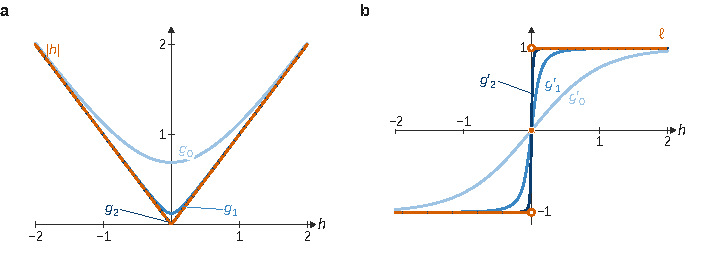
\includegraphics{figures/q18-convergence-derivees.pdf}
\caption*{Figure 3 --- (a) g\_β → \textbar h\textbar{} simplement ; (b) les g\_β′,
continues et nulles en 0, tendent vers ℓ, discontinue en 0 (tracé pour β
= 0, 1, 2)}
\end{figure}

\begin{center}\rule{0.5\linewidth}{0.5pt}\end{center}

\hypertarget{troisiuxe8me-partie}{%
\section{Troisième partie}\label{troisiuxe8me-partie}}

\hypertarget{question-19}{%
\subsection{Question 19}\label{question-19}}

Posons \(p=\frac{1+x}2\) et \(q=\frac{1-x}2\), de sorte que \(I(x)=p\ln p+q\ln q\).

Quand \(x\to1^-\), \(p\to1\) donc \(p\ln p\to0\), et \(q\to0^+\) donc \(q\ln q\to0\) (croissances comparées).

\(I\) étant paire, il en va de même en \(-1^+\).

\textbf{\(I\) se prolonge par continuité en posant \(I(\pm1)=0\)}, et devient continue sur \([-1,1]\).

\hypertarget{question-20}{%
\subsection{Question 20}\label{question-20}}

Soit \(K\) le nombre d'indices \(i\leqslant N\) tels que \(\sigma_i=1\).

On a \(K=\sum_i\frac{1+\sigma_i}2\), somme de \(N\) variables de Bernoulli de paramètre \(\frac12\) mutuellement indépendantes, donc \(K\sim\mathcal B(N,\frac12)\).

Comme \(\sum_i\sigma_i=K-(N-K)\),
\equationajustee{S_N=\frac{2K-N}N=-1+\frac{2K}N .}
\(S_N\) prend donc ses valeurs dans \(\mathscr M_N\), et \(S_N=x\) équivaut à \(K=\frac{N(1+x)}2\). D'où
\equationajustee{\boxed{P[S_N=x]=\begin{cases}\dbinom{N}{\frac{N(1+x)}2}2^{-N}&\text{si }x\in\mathscr M_N,\\[2mm]0&\text{sinon.}\end{cases}}}

\hypertarget{question-21}{%
\subsection{Question 21}\label{question-21}}

Posons \(m_N=\frac{N(1+u_N)}2\) : comme \(u_N\in\mathscr M_N\), c'est un entier de \(\{0,\dots,N\}\).

Posons aussi \(p_N=\frac{m_N}N=\frac{1+u_N}2\) et \(q_N=1-p_N\).

Alors \(p_N\to p=\frac{1+x}2\in\,]0,1[\) et \(q_N\to q=1-p\).

\emph{Les arguments des factorielles tendent vers l'infini.} \(m_N=Np_N\) et \(N-m_N=Nq_N\) avec \(p,q>0\), donc \(m_N\to+\infty\) et \(N-m_N\to+\infty\).

\emph{Stirling sans sommer d'équivalents.} De \(n!\sim\sqrt{2\pi n}\,(n/e)^n\) on tire, en passant au logarithme (si \(a_n\sim b_n\), alors \(\ln a_n-\ln b_n=\ln\frac{a_n}{b_n}\to0\)) :
\equationajustee{\ln n!=n\ln n-n+\tfrac12\ln(2\pi n)+o(1).}
On l'applique à \(N\), \(m_N\) et \(N-m_N\), qui tendent tous vers l'infini, et on \textbf{soustrait des égalités} (et non des équivalents). Les termes \(-n\) se compensent et les termes \(\frac12\ln(2\pi\,\cdot)\) sont des \(O(\ln N)\) :
\equationajustee{\ln\binom N{m_N}=N\ln N-m_N\ln m_N-(N-m_N)\ln(N-m_N)+O(\ln N).}
Avec \(\ln m_N=\ln N+\ln p_N\) et \(\ln(N-m_N)=\ln N+\ln q_N\), les termes en \(\ln N\) se compensent :
\equationajustee{\begin{aligned}
\frac1N\ln\binom N{m_N}&=-p_N\ln p_N-q_N\ln q_N+O\Big(\frac{\ln N}N\Big)\\
&\longrightarrow-p\ln p-q\ln q=-I(x),
\end{aligned}}
par continuité de \(u\mapsto u\ln u\) sur \(]0,1[\). Par Q20,
\equationajustee{-\frac1N\ln P[S_N=u_N]=-\frac1N\ln\binom N{m_N}+\ln2,}
donc
\equationajustee{\boxed{\lim_{N\to+\infty}-\frac1N\ln P[S_N=u_N]=I(x)+\ln2}}
\textbf{L'énoncé, qui annonce \(I(x)\), comporte une erreur de constante.}

Contrôle en \(x=0\) (avec \(u_N\in\{0,\frac1N\}\)) : \(P[S_N=u_N]\) est de l'ordre de \(\sqrt{2/(\pi N)}\) et ne décroît pas exponentiellement.

La limite vaut donc \(0=I(0)+\ln2\), alors que \(I(0)=-\ln2\). Le résultat annoncé serait exact avec
\equationajustee{J(x)=I(x)+\ln2=\frac{1+x}2\ln(1+x)+\frac{1-x}2\ln(1-x).}

\hypertarget{question-22}{%
\subsection{Question 22}\label{question-22}}

Soit \(x\in\mathscr M_N\). \(S_N\) prend ses valeurs dans l'ensemble fini \(\mathscr M_N\), donc, par la formule de transfert,
\equationajustee{Y_N(\beta,h)=\sum_{y\in\mathscr M_N}P[S_N=y]\,e^{N(\beta y^2+hy)} .}
C'est une somme finie de termes positifs, donc elle majore chacun d'eux :
\equationajustee{Y_N(\beta,h)\geqslant P[S_N=x]\,e^{N(\beta x^2+hx)}.}
Comme \(P[S_N=x]>0\) (Q20), on prend le logarithme (croissant) et on divise par \(N\) :
\equationajustee{\boxed{G_N(\beta,h)\geqslant\beta x^2+hx+\frac1N\ln P[S_N=x]}}
Compte tenu de Q21, la convergence admise est exacte sous la forme \(G_N(\beta,h)\to g(\beta,h)-\ln2\), avec \(g\) défini comme dans l'énoncé ; seule cette forme sert en Q30.

\hypertarget{question-23}{%
\subsection{Question 23}\label{question-23}}

Sur \(]-1,1[\), on dérive les deux termes de \(I\) :
\equationajustee{\begin{aligned}
I'(x)&=\tfrac12\ln\tfrac{1+x}2+\tfrac12-\tfrac12\ln\tfrac{1-x}2-\tfrac12\\
&=\tfrac12\ln\frac{1+x}{1-x},
\end{aligned}}
puis
\equationajustee{\begin{aligned}
I''(x)&=\frac12\Big(\frac1{1+x}+\frac1{1-x}\Big)\\
&=\frac1{1-x^2}.
\end{aligned}}
Donc, indépendamment de \(h\),
\equationajustee{\psi_{\beta,h}''(x)=2\beta-\frac1{1-x^2}.}

\begin{itemize}
\tightlist
\item
  Si \(\beta\in[0,\frac12]\) : \(\frac1{1-x^2}\geqslant1\geqslant2\beta\), donc \textbf{\(\psi''_{\beta,h}(x)\leqslant0\) pour tout \(x\in\,]-1,1[\)} (avec égalité seulement pour \(\beta=\frac12\) et \(x=0\)).
\item
  Si \(\beta>\frac12\) : \(\psi''_{\beta,h}(x)\leqslant0\) équivaut à \(1-x^2\leqslant\frac1{2\beta}\), c'est-à-dire, avec \(x\in\,]-1,1[\), \equationajustee{\boxed{|x|\geqslant\sqrt{1-\frac1{2\beta}}}}
\end{itemize}

\hypertarget{question-24}{%
\subsection{Question 24}\label{question-24}}

Soient \(\beta\geqslant0\) et \(h>0\). \(\psi=\psi_{\beta,h}\) est continue sur le segment \([-1,1]\) (Q19), donc atteint son maximum.

\emph{Localisation.} \(\beta x^2\) et \(I\) sont paires, donc pour \(x\in\,]0,1]\),
\equationajustee{\psi(x)-\psi(-x)=2hx>0 :}
aucun point de \([-1,0[\) n'est point de maximum. Sur \(]-1,1[\),
\equationajustee{\psi'(x)=2\beta x+h-\frac12\ln\frac{1+x}{1-x}.}
- D'une part \(\psi'(0)=h>0\), donc \(\psi\) croît strictement au voisinage de \(0\) : \(0\) n'est pas un maximum.
- D'autre part \(\psi'(x)\to-\infty\) quand \(x\to1^-\). Il existe donc \(a<1\) tel que \(\psi'<0\) sur \([a,1[\).
- Alors \(\psi\), continue en \(1\), est strictement décroissante sur \([a,1]\) : \(1\) n'est pas un maximum.

Tout point de maximum est donc dans l'ouvert \(]0,1[\), où \(\psi\) est dérivable : il annule \(\psi'\).

\emph{Unicité.} Sur \(]0,1[\),
\equationajustee{\psi'''(x)=-I'''(x)=-\frac{2x}{(1-x^2)^2}<0 .}
\(\psi''\) est donc strictement décroissante sur \([0,1[\), et \(\psi'\) y est \textbf{strictement concave} (argument de Q6, avec des inégalités strictes).

Supposons que \(\psi'\) s'annule en \(0<z_1<z_2<1\). Écrivons \(z_1=t\cdot0+(1-t)z_2\) avec \(t\in\,]0,1[\). La stricte concavité donne
\equationajustee{\begin{aligned}
0=\psi'(z_1)&>t\,\psi'(0)+(1-t)\,\psi'(z_2)\\
&=th>0,
\end{aligned}}
ce qui est absurde. \(\psi'\) a donc au plus un zéro dans \(]0,1[\), et au moins un (le point de maximum).

\textbf{\(\psi_{\beta,h}\) atteint son maximum en un unique point \(x_*(\beta,h)\in\,]0,1[\)}, caractérisé par \(\psi'_{\beta,h}(x_*)=0\).

De plus \(\psi'>0\) sur \([0,x_*[\) et \(\psi'<0\) sur \(]x_*,1[\).

\emph{Cas \(h<0\).} On a \(\psi_{\beta,h}(x)=\psi_{\beta,-h}(-x)\). Donc \(\psi_{\beta,h}\) atteint son maximum en un unique point, à savoir \(-x_*(\beta,-h)\in\,]-1,0[\).

\hypertarget{question-25}{%
\subsection{Question 25}\label{question-25}}

Ici \(h=0\) : \(\psi_{\beta,0}(x)=\beta x^2-I(x)\) est paire et \(\psi'_{\beta,0}(0)=0\).

\emph{Cas \(\beta\in[0,\frac12]\).} Par Q23, \(\psi''_{\beta,0}<0\) sur \(]-1,1[\), sauf éventuellement en \(0\).

\(\psi'_{\beta,0}\) est donc strictement décroissante. Nulle en \(0\), elle est \(>0\) sur \(]-1,0[\) et \(<0\) sur \(]0,1[\).

Par continuité de \(\psi_{\beta,0}\) en \(\pm1\), \(\psi_{\beta,0}\) est strictement croissante sur \([-1,0]\) et strictement décroissante sur \([0,1]\).

\textbf{Le maximum est atteint en \(0\) et seulement en \(0\).}

\emph{Cas \(\beta>\frac12\).} Sur \([0,1[\), \(\psi'_{\beta,0}\) est strictement concave (même calcul qu'en Q24). On dispose de :

\begin{itemize}
\tightlist
\item
  \(\psi'_{\beta,0}(0)=0\) et \(\psi''_{\beta,0}(0)=2\beta-1>0\), donc il existe \(\varepsilon\in\,]0,1[\) avec \(\psi'_{\beta,0}(\varepsilon)>0\) ;
\item
  \(\psi'_{\beta,0}(x)\to-\infty\) quand \(x\to1^-\).
\end{itemize}

Par le théorème des valeurs intermédiaires, \(\psi'_{\beta,0}\) s'annule en un point \(c\in\,]\varepsilon,1[\).

Ce zéro est unique dans \(]0,1[\).

En effet, une fonction strictement concave s'annule au plus deux fois : si \(a<b<c'\) étaient trois zéros, \(b\) serait combinaison convexe stricte de \(a\) et \(c'\), et la stricte concavité donnerait \(0>0\). Or \(0\) est déjà un zéro.

Entre ses zéros, \(\psi'_{\beta,0}\) garde un signe constant (valeurs intermédiaires). Elle est \(>0\) en \(\varepsilon<c\) et tend vers \(-\infty\) en \(1^-\).

Donc \(\psi'_{\beta,0}>0\) sur \(]0,c[\) et \(\psi'_{\beta,0}<0\) sur \(]c,1[\).

Ainsi \(\psi_{\beta,0}\) est strictement croissante sur \([0,c]\) et strictement décroissante sur \([c,1]\) : sur \([0,1]\), le maximum est atteint en \(c\) seul.

Par parité, sur \([-1,1]\), \textbf{le maximum est atteint exactement en \(x_*(\beta,0):=c\in\,]0,1[\) et en \(-x_*(\beta,0)\).}

\begin{figure}[H]
\centering
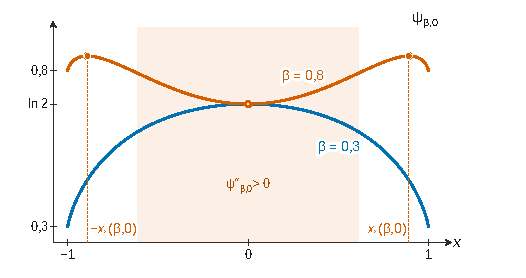
\includegraphics{figures/q25-profil-psi.pdf}
\caption*{Figure 4 --- Profil ψ\_β,0 : maximum unique en 0 pour β = 0,3 ; pour β =
0,8, 0 devient un minimum local (zone teintée : ψ″ \textgreater{} 0) et
les maxima sont en ±x*(β, 0)}
\end{figure}

\hypertarget{question-26}{%
\subsection{Question 26}\label{question-26}}

Comme \(v_n\to h>0\), il existe \(n_1\) tel que \(v_n>0\) pour \(n\geqslant n_1\).

Posons alors \(x_n=x_*(\beta,v_n)\in\,]0,1[\) et \(\ell=\lim x_n\), qui appartient au fermé \([0,1]\).

\emph{Caractère maximal.} Pour \(n\geqslant n_1\) et tout \(y\in[-1,1]\),
\equationajustee{\beta x_n^2+v_nx_n-I(x_n)\geqslant\beta y^2+v_ny-I(y).}

\emph{Passage à la limite.} \(I\) est continue sur \([-1,1]\) (Q19), y compris aux bords, où \(\ell\) peut se trouver a priori. Avec \(x_n\to\ell\) et \(v_n\to h\), on obtient, pour tout \(y\in[-1,1]\),
\equationajustee{\psi_{\beta,h}(\ell)\geqslant\psi_{\beta,h}(y).}

\emph{Unicité.} \(\ell\) est un point de maximum de \(\psi_{\beta,h}\) ; par l'unicité de Q24,
\equationajustee{\boxed{\lim_{n\to\infty}x_*(\beta,v_n)=x_*(\beta,h)}}

\hypertarget{question-27}{%
\subsection{Question 27}\label{question-27}}

Pour \(h\geqslant0\), \(x_*(\beta,h)\) est un point de maximum de \(\psi_{\beta,h}\) sur \([-1,1]\).

C'est Q24 si \(h>0\), et Q25 si \(h=0\), que \(\beta\) soit au-dessous ou au-dessus de \(\frac12\).

Le supremum \(g(\beta,h)\) est donc atteint :
\equationajustee{g(\beta,h)=\psi_{\beta,h}\big(x_*(\beta,h)\big).}
Posons \(x_*=x_*(\beta,h)\) et comparons \(\psi_{\beta,h'}\) et \(\psi_{\beta,h}\) : \(\psi_{\beta,h'}(x)=\psi_{\beta,h}(x)+(h'-h)x\). Comme \(g(\beta,h')\) majore \(\psi_{\beta,h'}\),
\equationajustee{\begin{aligned}
g(\beta,h')&\geqslant\psi_{\beta,h'}(x_*)\\
&=\psi_{\beta,h}(x_*)+(h'-h)x_*\\
&=g(\beta,h)+(h'-h)x_*.
\end{aligned}}
En échangeant les rôles de \(h\) et \(h'\) :
\equationajustee{g(\beta,h)\geqslant g(\beta,h')+(h-h')\,x_*(\beta,h').}
D'où
\equationajustee{\boxed{(h'-h)\,x_*(\beta,h)\leqslant g(\beta,h')-g(\beta,h)\leqslant(h'-h)\,x_*(\beta,h')}}

\hypertarget{question-28}{%
\subsection{Question 28}\label{question-28}}

Soit \(h>0\) et \(h'\geqslant0\) avec \(h'\neq h\). On divise l'encadrement de Q27 par \(h'-h\), en renversant les inégalités si \(h'<h\) : le taux
\equationajustee{\tau(h')=\frac{g(\beta,h')-g(\beta,h)}{h'-h}}
est compris entre \(x_*(\beta,h)\) et \(x_*(\beta,h')\).

Par la continuité admise de \(h'\mapsto x_*(\beta,h')\) sur \([0,+\infty[\), \(x_*(\beta,h')\to x_*(\beta,h)\) quand \(h'\to h\).

Par encadrement, \(\tau(h')\to x_*(\beta,h)\) :
\equationajustee{\boxed{h'\mapsto g(\beta,h')\text{ est \text{dérivable} en }h\text{ et }\frac{\partial g}{\partial h}(\beta,h)=x_*(\beta,h)}}

\hypertarget{question-29}{%
\subsection{Question 29}\label{question-29}}

\emph{Parité.} \(\psi_{\beta,-h}(x)=\psi_{\beta,h}(-x)\) et \([-1,1]\) est symétrique, donc \(g(\beta,-h)=g(\beta,h)\).

\emph{Hors de \(0\).} \(g(\beta,\cdot)\) est dérivable sur \(]0,+\infty[\) (Q28), donc sur \(]-\infty,0[\) par parité (composée avec \(h\mapsto-h\)).

\emph{En \(0\).} Q27 avec \(h=0\) et \(h'>0\) donne
\equationajustee{x_*(\beta,0)\leqslant\frac{g(\beta,h')-g(\beta,0)}{h'}\leqslant x_*(\beta,h').}
Par la continuité admise en \(0\), la dérivée à droite en \(0\) existe et vaut \(x_*(\beta,0)\). Par parité, la dérivée à gauche vaut \(-x_*(\beta,0)\).

Donc \(g(\beta,\cdot)\) est dérivable en \(0\) si et seulement si \(x_*(\beta,0)=0\), c'est-à-dire, par Q25, si et seulement si \(\beta\leqslant\frac12\) :
\equationajustee{\boxed{h\mapsto g(\beta,h)\text{ est \text{dérivable} sur }\mathbb R\iff\beta\in\big[0,\tfrac12\big]}}

\begin{figure}[H]
\centering
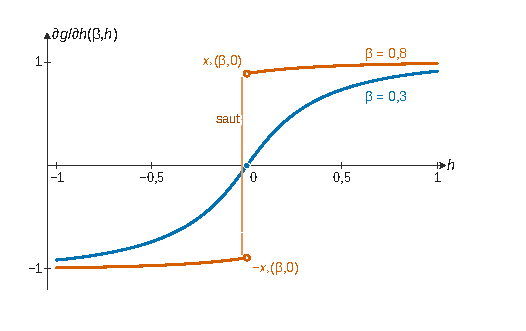
\includegraphics{figures/q29-aimantation-saut.pdf}
\caption*{Figure 5 --- Dérivée ∂g/∂h (β, h) en fonction de h : continue pour β =
0,3, saut de −x\emph{(β, 0) à x}(β, 0) en h = 0 pour β = 0,8}
\end{figure}

\hypertarget{question-30}{%
\subsection{Question 30}\label{question-30}}

On a \(\frac\beta N\sum_{i,j}\sigma_i\sigma_j=\frac\beta N\big(\sum_i\sigma_i\big)^2=\beta NS_N^2\) et \(h\sum_i\sigma_i=hNS_N\). La quantité étudiée vaut donc
\equationajustee{Q_N=\frac{E\big[S_N\,e^{\beta NS_N^2+hNS_N}\big]}{Y_N(\beta,h)} .}
\(Y_N\) est une somme finie de fonctions dérivables en \(h\) (Q22), et
\equationajustee{\begin{aligned}
Q_N&=\frac1N\,\frac{\partial_hY_N(\beta,h)}{Y_N(\beta,h)}\\
&=\frac{\partial G_N}{\partial h}(\beta,h).
\end{aligned}}
Vérifions les hypothèses de Q4 pour \(f_N=G_N(\beta,\cdot)+\ln2\) :

\begin{itemize}
\tightlist
\item
  avec \(W^{(N)}=(NS_N^2,NS_N)\), à valeurs dans un ensemble fini de \(\mathbb R^2\), \(\ln Y_N(\beta,h)=\phi_{W^{(N)}}(\beta,h)\) est convexe (Q8) ; donc \(f_N\) est convexe et dérivable sur \(\mathbb R\) ;
\item
  par la convergence admise, sous sa forme rectifiée (Q21--Q22), \(f_N\to g(\beta,\cdot)\) simplement sur \(\mathbb R\) ;
\item
  \(g(\beta,\cdot)\) est dérivable en \(h>0\), de dérivée \(x_*(\beta,h)\) (Q28).
\end{itemize}

La question 4 donne \(f_N'(h)=Q_N\to x_*(\beta,h)\) :
\equationajustee{\boxed{\lim_{N\to+\infty}\frac1{Y_N(\beta,h)}E\Big[\Big(\frac1N\sum_{i=1}^N\sigma_i\Big)\exp\Big(\frac\beta N\sum_{i,j}\sigma_i\sigma_j+h\sum_i\sigma_i\Big)\Big]=x_*(\beta,h)}}
La constante \(\ln2\) est sans effet : l'énoncé tel qu'admis conduirait à la même dérivée.

\hypertarget{question-31}{%
\subsection{Question 31}\label{question-31}}

Par Q24, \(x_*=x_*(\beta,h)\in\,]0,1[\) annule \(\psi'_{\beta,h}\) :
\equationajustee{\frac12\ln\frac{1+x_*}{1-x_*}=h+2\beta x_* .}
Or, pour \(t\in\mathbb R\) et \(x\in\,]-1,1[\),
\equationajustee{\begin{aligned}
\operatorname{th}t=x&\iff\frac{e^{2t}-1}{e^{2t}+1}=x\\
&\iff e^{2t}=\frac{1+x}{1-x}\\
&\iff t=\frac12\ln\frac{1+x}{1-x}.
\end{aligned}}
Avec \(t=h+2\beta x_*\) :
\equationajustee{\boxed{x_*(\beta,h)=\operatorname{th}\big(h+2\beta x_*(\beta,h)\big)}}

\begin{figure}[H]
\centering
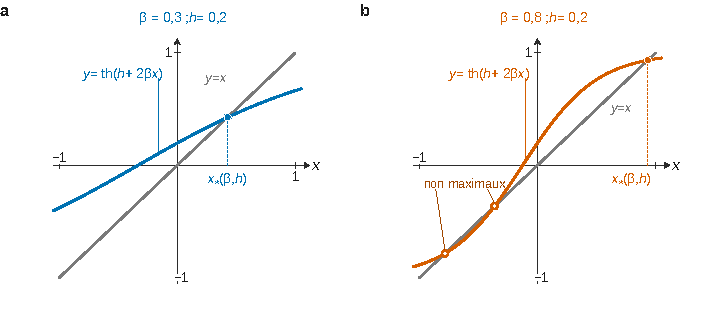
\includegraphics{figures/q31-point-fixe.pdf}
\caption*{Figure 6 --- Pour h = 0,2, x*(β, h) est l'abscisse de l'intersection
positive de y = x et y = th(h + 2βx) ; pour β = 0,8, les deux
intersections négatives ne sont pas des maxima}
\end{figure}

\hypertarget{question-32}{%
\subsection{Question 32}\label{question-32}}

Notons \(x_h=x_*(\frac12,h)\) pour \(h>0\). Par Q24 et Q31, \(x_h\in\,]0,1[\) et \(\frac12\ln\frac{1+x_h}{1-x_h}=h+x_h\), soit \(\Phi(x_h)=h\) avec
\equationajustee{\Phi(x)=\frac12\ln\frac{1+x}{1-x}-x .}

\emph{\(x_h\) tend vers \(0\).} Sur \(]0,1[\),
\equationajustee{\Phi'(x)=\frac1{1-x^2}-1=\frac{x^2}{1-x^2}>0 .}
\(\Phi\) est donc une bijection continue strictement croissante de \([0,1[\) sur \([0,+\infty[\) (car \(\Phi(0)=0\) et \(\Phi\to+\infty\) en \(1\)), de réciproque continue.

Donc \(x_h=\Phi^{-1}(h)\to\Phi^{-1}(0)=0\) quand \(h\to0^+\).

(On peut aussi invoquer la continuité admise et \(x_*(\frac12,0)=0\), par Q25.)

\emph{Équivalent.} Par différence des développements en série entière de \(\ln(1+x)\) et \(\ln(1-x)\), pour \(|x|<1\),
\equationajustee{\frac12\ln\frac{1+x}{1-x}=\sum_{k\geqslant0}\frac{x^{2k+1}}{2k+1}.}
Donc \(\Phi(x)=\frac{x^3}3+O(x^5)\), d'où \(\Phi(x)\sim\frac{x^3}3\) en \(0\).

Comme \(x_h\to0\), on peut composer : \(h=\Phi(x_h)\sim\frac{x_h^3}3\), soit \(\frac{x_h^3}{3h}\to1\).

Par continuité de \(t\mapsto t^{1/3}\) en \(1\) :
\equationajustee{\boxed{\lim_{\substack{h\to0\\h>0}}\frac{x_*(\frac12,h)}{(3h)^{1/3}}=1}}

\end{document}
